\section{Methodology}\label{sec:method}

We analyzed not only the code, but also the metadata linked to it. The research process had four steps: choosing the AIDev version, enriching developer profiles with GitHub activity data, splitting users into groups, and comparing agent use between these groups. Results at the pull-request level were aggregated per developer, to avoid treating several contributions from the same person as independent observations.

\subsection{Data sources and sample construction}

We use the Zenodo v3 release of the AIDev dataset (DOI \texttt{10.5281/zenodo.16919272}), described in Section 1.

Activity in AIDev mostly describes developers with respect to their agent-related contributions. To get a wider range of information, we enriched the records using the GitHub GraphQL API. Table~\ref{tab:profile-indicators} shows the 12 quantitative indicators used for clustering. The five-year indicators cover the five years before the data collection. GitHub only provides an aggregated count of contributions to private repositories (not only commits, and only for users who agreed to show this) - this should not be read as an exact count of private commits. During data collection, a login was treated as unavailable - deleted, renamed, or unavailable for some other reason - whenever the API returned a status other than 200. The corresponding developers are exactly those whose indicators were later estimated using the random-forest method described below. GraphQL data collection took place on 6 May 2026. Note that this is about 9 months after the period covered by the AIDev data, and these values may have changed in that time.

GraphQL data collection returned activity records for 70\,434 of 72\,189 developers (97.57\%). The numeric indicators for the remaining 1755 developers were estimated using random-forest regression models \cite{breiman2001random}. The models were evaluated with an 80/20 train/test split, and the predicted numeric values were rounded to whole numbers. Their predictive performance was limited - the observed $R^2$ values are shown in Table~\ref{tab:r2-values}. These values should therefore be treated as an approximate way to fill in missing profiles, not as a reliable reconstruction of their activity.

\begin{table}[H]
    \centering
    \caption{Predictive performance ($R^2$) of the random-forest imputation models.}
    \label{tab:r2-values}
    \small
    \begin{tabular}{lr}
        \toprule
        \textbf{Indicator} & \textbf{$R^2$} \\
        \midrule
        \texttt{collab\_breadth} & 0.098 \\
        \texttt{5yr\_prs\_opened} & 0.088 \\
        \texttt{5yr\_reviews\_given} & 0.020 \\
        \texttt{5yr\_public\_commits} & $-0.073$ \\
        \texttt{5yr\_private\_work} & $-0.272$ \\
        \bottomrule
    \end{tabular}
\end{table}
\begin{table}[H]
    \centering
    \caption{Indicators used to build developer activity profiles.}
    \label{tab:profile-indicators}
    \small
    \begin{tabularx}{\linewidth}{@{}p{0.31\linewidth}X@{}}
        \toprule
        \textbf{Indicator} & \textbf{Operationalization} \\
        \midrule
        Collaboration breadth & Number of repositories the developer contributed to. \\
        Public commits & Public commit-type contributions in the preceding five years. \\
        Private activity & Private contributions in the preceding five years, when disclosed by GitHub. \\
        Opened pull requests & Pull requests opened in the preceding five years. \\
        Reviews submitted & Pull-request reviews submitted in the preceding five years. \\
        Account age & Time elapsed since the GitHub account was created. \\
        Followers & Number of followers at the time of data collection. \\
        Maximum stars & Highest number of stars among the developer's repositories. \\
        Maximum forks & Highest number of forks among the developer's repositories. \\
        Agentic-PR activity span & Number of days between the developer's first and last Agentic-PR. \\
        Agent diversity & Number of different coding agents used in the developer's Agentic-PRs. \\
        Agentic-PR repository range & Number of different repositories in which the developer has an Agentic-PR. \\
        \bottomrule
    \end{tabularx}
\end{table}

\subsection{Preprocessing and activity-profile construction}

The indicators were strongly right-skewed and differed by several orders of magnitude. We applied a log(1+x) transformation, and then standardized each feature to zero mean and unit variance. We then used Isolation Forest with the contamination parameter set to 1\%, to remove the most extreme cases \cite{liu2008isolation}. This procedure removed 722 developers, leaving 71\,467 profiles for the main analysis.

A quantile transformation toward a normal marginal distribution was tried first instead of log(1+x), but a complete-case sensitivity check (Section 5) showed that it was unstable. Clustering on data containing only developers with real GraphQL data agreed with clustering on the full population at only an Adjusted Rand Index of 0.46. The same check with log(1+x) gave an Adjusted Rand Index of 0.98, so we kept this second method.

Principal component analysis was computed on the transformed indicators to help interpret the dominant axes of variation, not as a dimensionality-reduction step feeding the clustering algorithm \cite{jolliffe2016principal}. The first two principal components keep only about 50\% of the variance, so a projection to 2 dimensions would discard roughly half of the information. We therefore ran clustering on the full, 12-dimensional, cleaned representation; we report PCA(2) separately, purely for visualization, to show which indicators drive the two dominant axes. As Figure~\ref{fig:pca-loadings} shows, the first component loads positively on activity indicators and can be read as a general activity axis. The second component contrasts agent-related activity and the size of public contributions against general recognition and review activity.

\begin{figure}[H]
    \centering
    
\includegraphics[width=0.92\linewidth]{pca_1.png}
    \vspace{0.5em}
    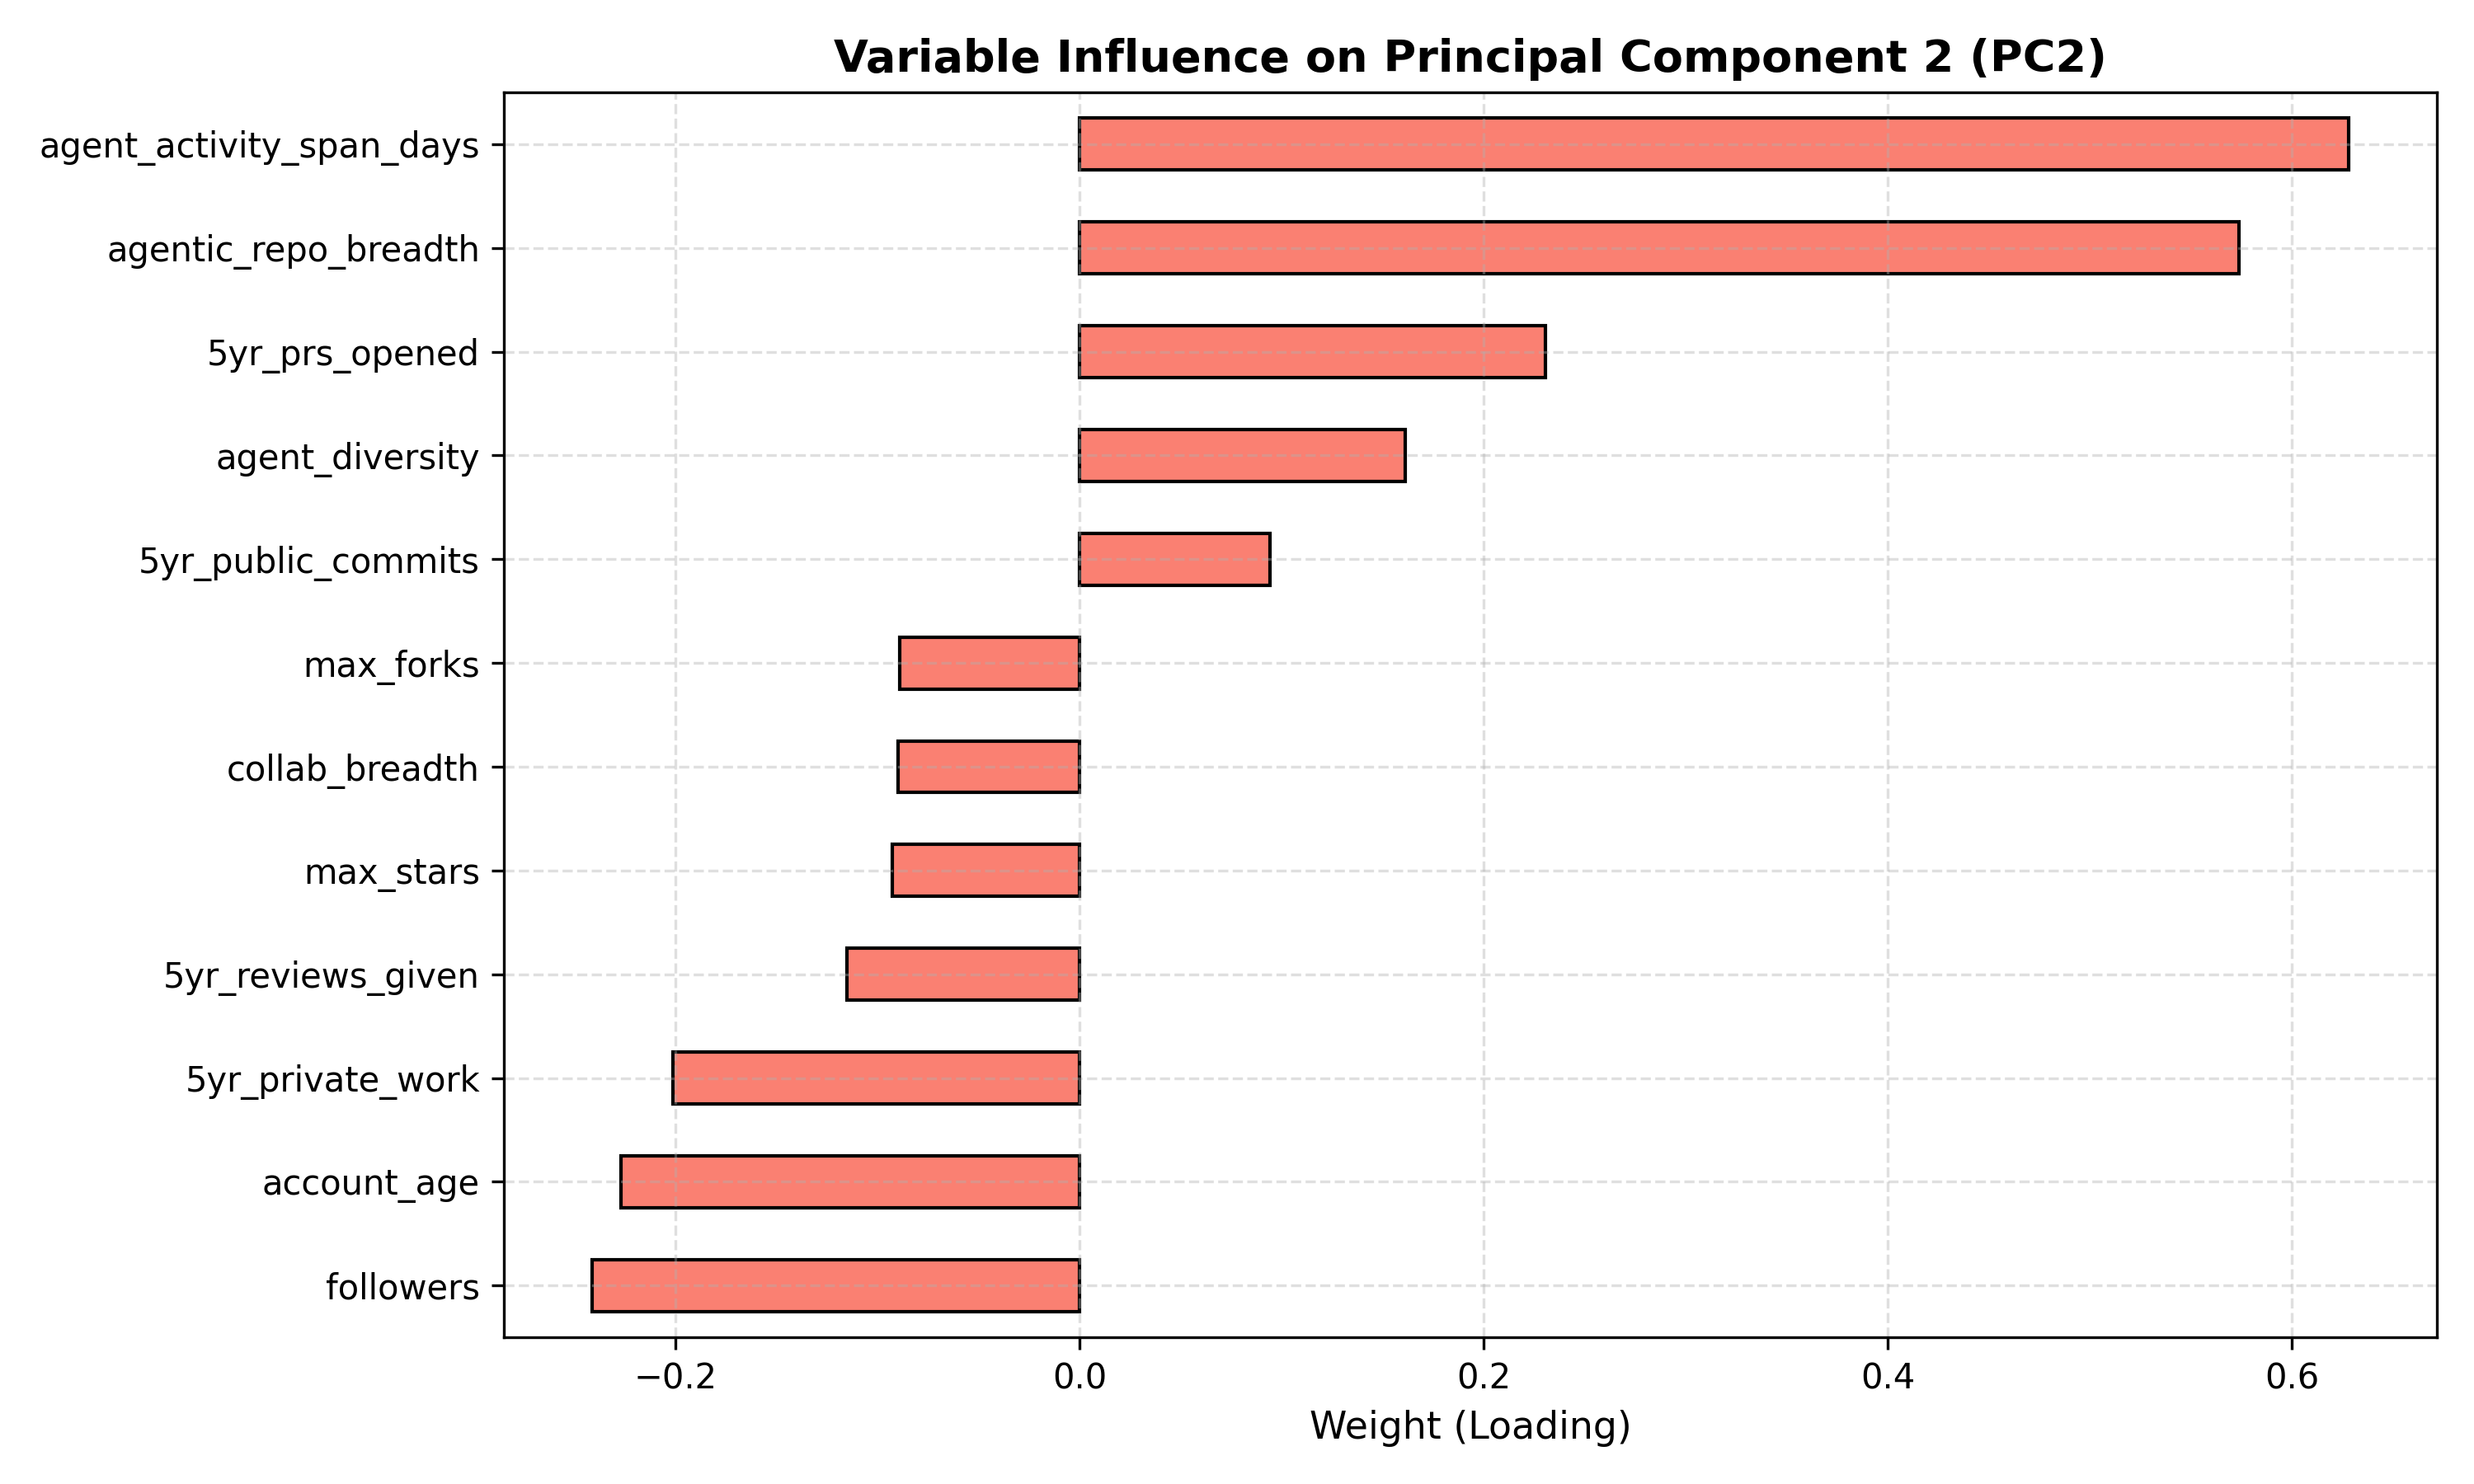
\includegraphics[width=0.92\linewidth]{pca_2.png}
    \caption{Loadings of the activity indicators on the two dominant axes of variation (PC1, PC2), computed only for interpretation purposes; PC1+PC2 keep about 50\% of the variance and are not used as clustering input. PC1 mainly represents general activity on GitHub, while PC2 contrasts agent-related activity and the size of public contributions against general recognition and review activity.}
    \label{fig:pca-loadings}
\end{figure}

We split the full, 12-dimensional, cleaned representation using $k$-means clustering \cite{lloyd1982least}. We also checked the results for different values of $k=2,\ldots,10$ using the average silhouette width \cite{rousseeuw1987silhouettes} and the gap statistic \cite{tibshirani2001gap}, computed on the same 12-dimensional representation. Figure~\ref{fig:cluster-diagnostics} shows that $k=3$ is not the numeric optimum under either statistic. Even so, we kept this value as a deliberately simple and interpretable parameter, matched to comparisons between low-, medium-, and high-activity profiles. The analysis is therefore conditional on this choice and does not assume that three clusters reflect the true underlying structure of the developer population.

\begin{figure}[H]
    \centering
    
\includegraphics[width=0.90\linewidth]{silnouette.png}
    \vspace{0.5em}
    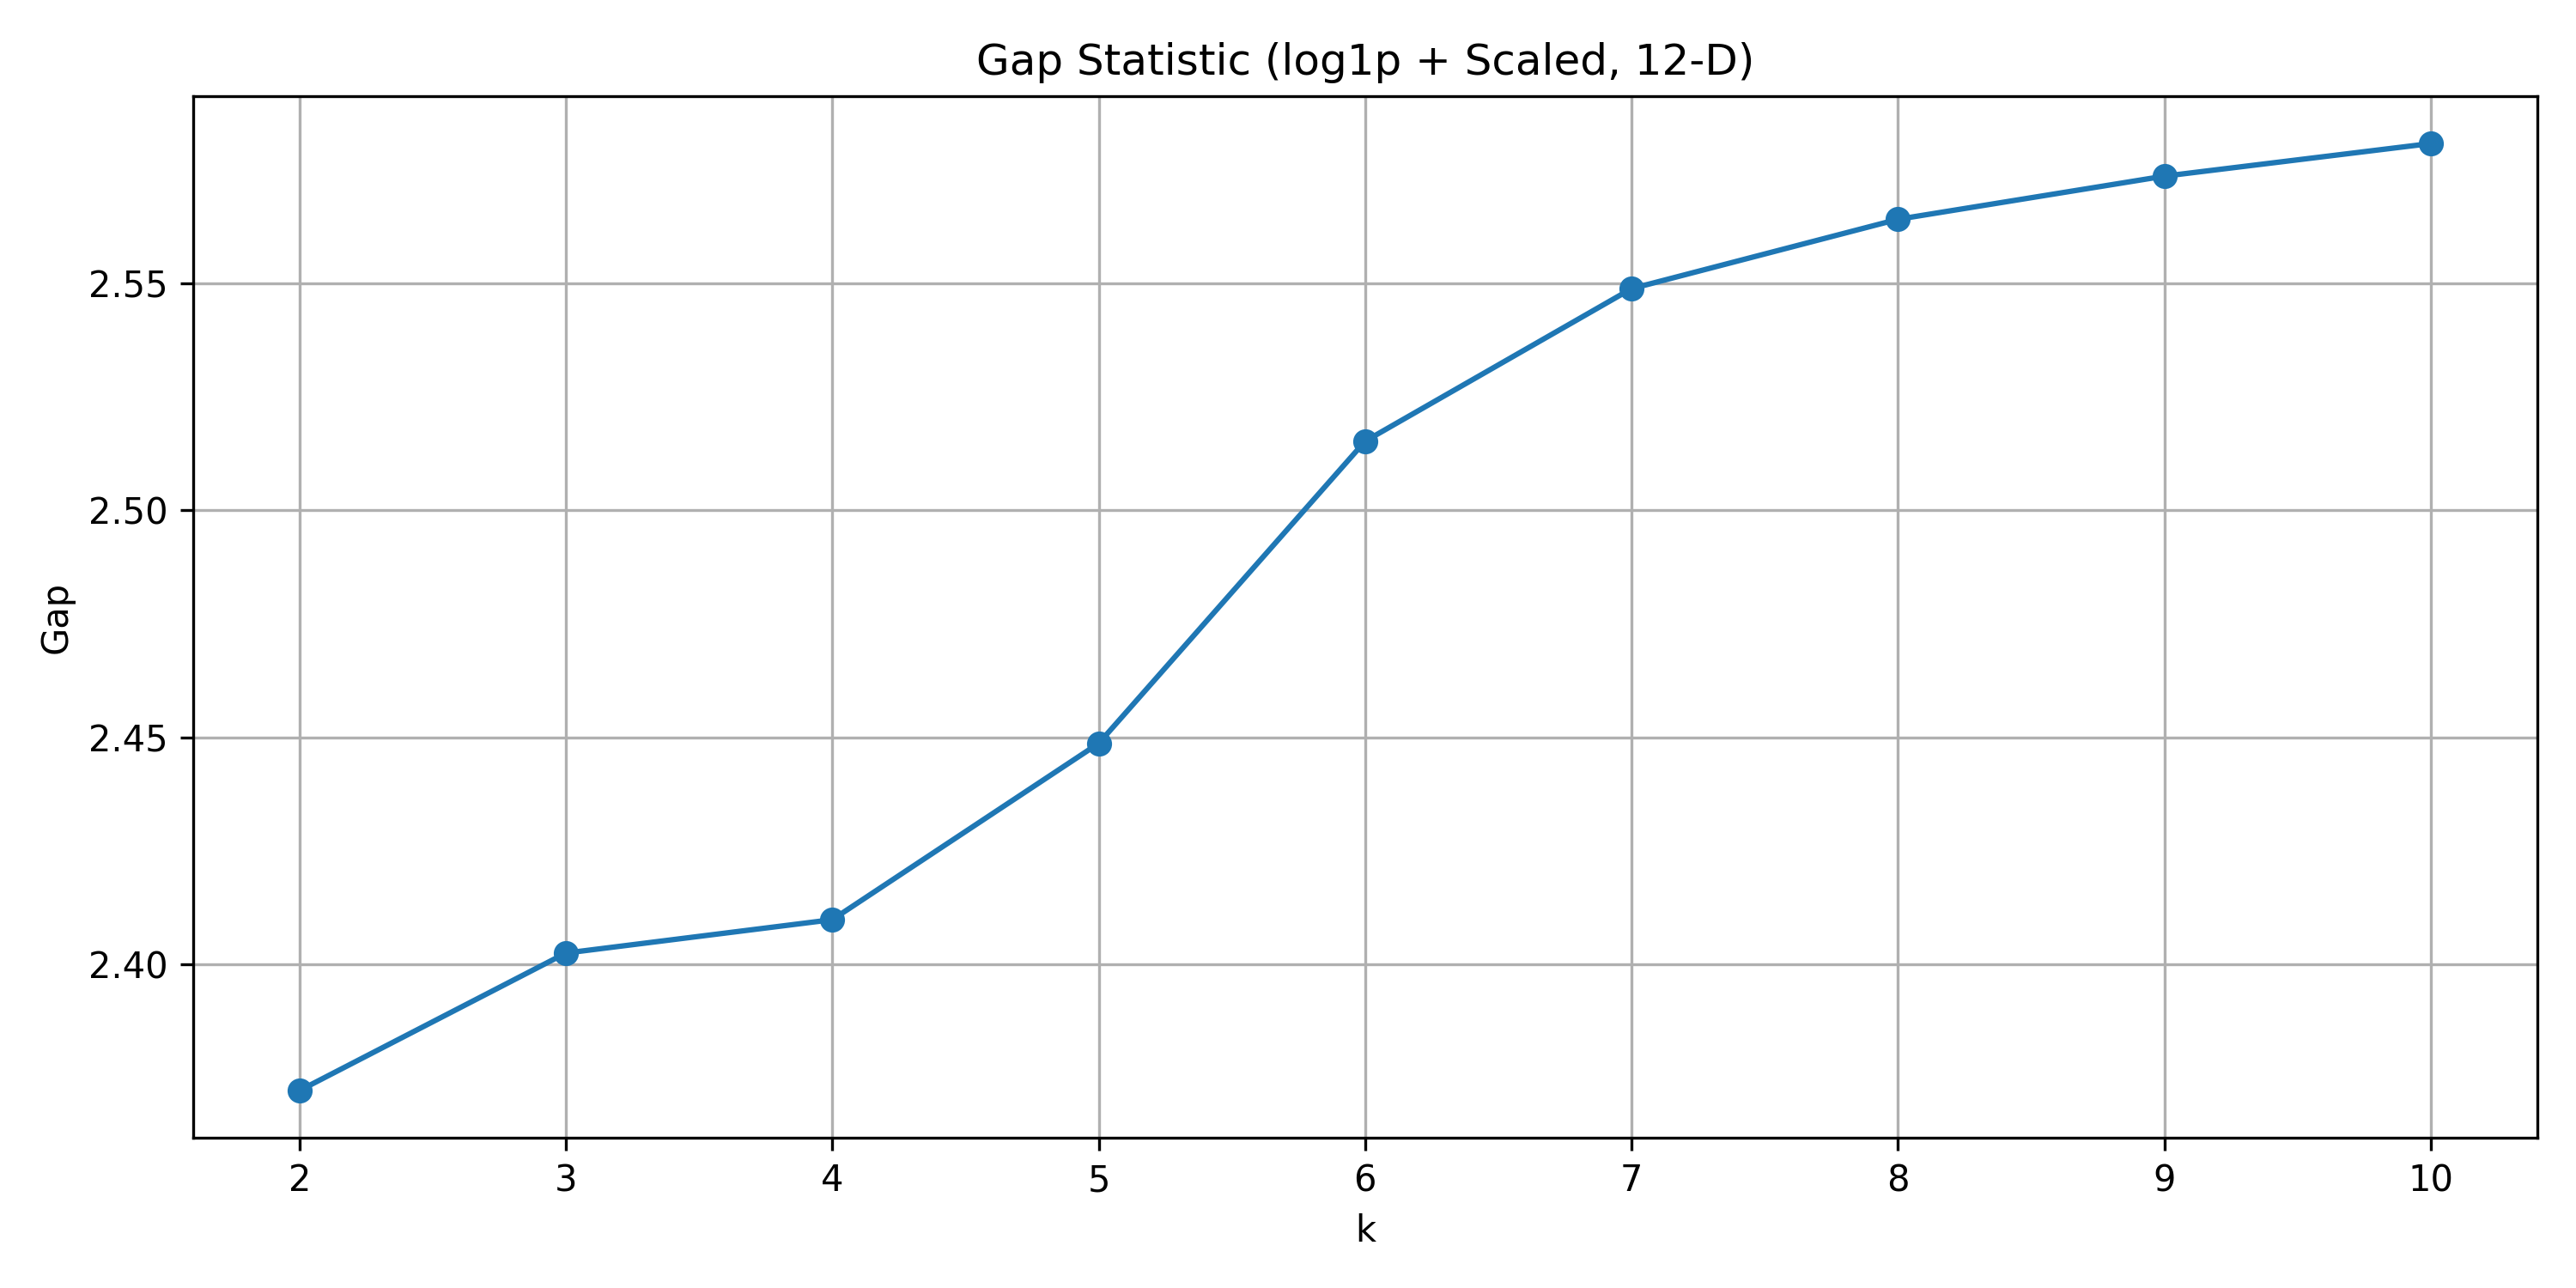
\includegraphics[width=0.90\linewidth]{gap_statistic.png}
    \caption{Silhouette-width and gap-statistic diagnostics for candidate values of $k$, computed on the 12-dimensional clustering input. $k=3$ is not the numeric optimum under either diagnostic; it is kept as a design choice driven by interpretability.}
    \label{fig:cluster-diagnostics}
\end{figure}

For readability, we call the low-, medium-, and high-activity profiles Junior, Mid, and Senior. They contain 44\,854, 12\,705, and 13\,908 developers respectively. These labels are not verified job titles, career stages, or direct measures of programming skill. This distinction matters concretely for RQ1: the Mid profile turns out to have the highest median number of Agentic-PRs among the three profiles (Section~\ref{sec:results}), even though it ranks lower than Senior in the combined activity score, because that score also reflects indicators (followers, account age, repository stars and forks) on which Senior scores higher.

\subsection{Outcome measures}

The outcome variables were not part of the clustering input.

\paragraph{RQ1: AI-agent use intensity.}
For each developer, we counted the number of Agentic-PRs linked to that developer in the full AIDev dataset. This variable measures the observed volume of contribution within the dataset's time window. It does not measure the share of a developer's total work done with an agent, nor the overall likelihood that a developer uses AI tools.

\paragraph{RQ2: pull-request acceptance.}
For each developer, we computed the share of resolved Agentic-PRs that were merged. A pull request was classified as merged when its \texttt{merged\_at} field was non-empty, and as rejected when it was closed without being merged. Open pull requests were excluded from the denominator, rather than being treated as rejected. Developers with no resolved Agentic-PR were excluded from this analysis. This outcome concerns pull-request acceptance, not the correctness of individual generated lines of code or its overall quality.

\paragraph{RQ3: Agentic-PR acceptance vs.\ a human-authored baseline.}
AIDev separately provides the \texttt{human\_pull\_request} table - a baseline sample of human-authored pull requests (with no agent involvement), taken from repositories with more than 500 stars. We first considered developers appearing in both groups, but found that only 351 of the 2515 distinct authors in \texttt{human\_pull\_request} were also among the 72\,189 developers linked to Agentic-PRs. This led to the decision that in RQ3 we compare two independent populations: the acceptance rate of all Agentic-PRs, summed across activity profiles, against the acceptance rate of \texttt{human\_pull\_request}, using the same merged/rejected/open classification as in RQ2. This is a population-level comparison, not matched at the developer level, and the baseline population is itself limited to a narrower sample of repositories than the full Agentic-PR population.

\subsection{Statistical analysis}
The distributions of the outcome variables could not be easily matched to common, well-known distributions, and the count-based measures contained many ties and zeros. For RQ1-RQ2, each of which compares three activity profiles, we first apply the Kruskal-Wallis test to check whether the outcome distributions differ between the three groups. A significant overall test result is followed up with two-sided pairwise Mann-Whitney $U$ tests, where the three pairwise comparisons for each research question are corrected with the Bonferroni correction, at a significance level of $\alpha=0.05$. RQ3 compares only two independent groups, so we use a single Mann-Whitney $U$ test, without an overall Kruskal-Wallis step and without a Bonferroni correction.

For each group we recorded the sample size, mean, standard deviation, and median. We further supplement the $p$-values with effect sizes: epsilon-squared for the Kruskal-Wallis test, and rank-biserial correlation for the pairwise comparisons. We report each effect size together with a 95\% confidence interval obtained through non-parametric bootstrapping: for epsilon-squared, we resample each group independently with replacement, recompute the Kruskal-Wallis statistic, and take the 2.5th and 97.5th percentiles from 2000 resampling runs. The same procedure, applied to the two compared groups, is used for each rank-biserial correlation in the pairwise comparisons. All analyses concern relationships between activity-based profiles and the observed outcomes.
